\documentclass{article}
\usepackage{fancyhdr}
\usepackage{graphicx}
\usepackage[german]{babel}
\pagestyle{fancy}

\author{Philipp Kiss}

\lhead{Philipp Kiss}
\rhead{Kommunikationstechnik}

\begin{document}
\section{OSI Modell}
Das OSI (Open Systems Interconnection) Modell umschreibt den Informationsaustausch zwischen zwei Systemen. Der Informationsaustausch wird in einem aus 7 Schichten bestehenden Stack modelliert. Protokolle definieren den Horizontalen Informationsaustausch (Von Sender Schicht \textit{n} zu Empfänger Schicht \textit{n}), wobei der reale Informationsfluss über die unterliegenden Schichten wandert und schlussendliche in der Layer 1, der Physical Layer, über ein Medium zur Layer 1 des Empfängers fliesst.
\subsection{``Layer 0'' - Medium}
Das Übertragungsmedium wird nicht wirklich zu den 7 Schichten gezählt, ich führe es hier als unterste Schicht auf, da dies dem schematischen Informationsfluss folgt. Generell gilt je grösser die Bandbreite, desto grösser die Übertragungsrate.
\subsubsection{Limitierungen}
Die Lichtgeschwindigkeit im Vakuum beträgt $c_0 = 299'792'458 \frac{m}{s} $. Es gibt keine praktische Anwendung in der der Informationsaustausch diese Geschwindigkeit $c_0$ übertrifft. In reinem Glas mit einem Brechungsindex von 1.5 beträgt die Geschwindigkeit $c_{Glas} = 200'000 \frac{km}{s} \left(= 20 \frac{cm}{ns} \right)$. Glücklicherweise beträgt die Ausbreitung eines elektrischen Signals in einem Leiter mit der typischen Permittivität $\varepsilon_r = 2.25$ ebenso $200'000 \frac{km}{s}$. Das sind die maximalen Geschwindigkeiten, die in der Praxis für Informationsübertragung erreicht werden kann.
\subsubsection{Signaldämpfung}
Für alle Übertragungsmedium stellt die Signaldämpfung ein Problem dar. Die Amplitude eines elektrischen wie auch eines optischen Signals nimmt mit steigender Übertragungsdistanz exponentiell ab. Da die absolute Störung auf ganzem Weg gleich bleibt, steigt das Verhältnis von Störung / Signal, wodurch das Signal ab einer Distanz nicht mehr eindeutig wahrnehmbar ist.

Berechnet wird die Dämpfung durch $A = 10 \cdot \log_{}(\frac{P_1}{P_2}) = 20 \cdot \log_{}(\left(\frac{U_1}{U_2}\right)^{2})$, und in Dezibel (dB) angegeben. Es gilt: eine Halbierung der Leistung bewirkt einer Dämpfung von 3 dB.
Die Signal to Noise Ration (SRN) wird durch $SRN = 10 \cdot \log_{}(\frac{P_{S}}{P_N})$(dB) definiert.
\newpage
\subsubsection{Elektrische Leiter}
Elektrische Leiter nutzen elektrische Impulse über metallene Leiter um ein Signal zu übertragen. Dabei ist zu beachten, dass elektrische Leiter durch elektromagnetische Störungen beeinflusst werden können und sie für eine brauchbare Signalübertragung davor geschützt werden müssen. Zudem muss ein elektrischer Leiter zwei sich nicht berührende Leiter anbieten, da ansonsten der Stromkreislauf nicht geschlossen werden kann und eine Signalübertragung verunmöglicht wird.
\paragraph{Koaxkabel}
eignen sich zur Übertragung hochfrequenter Signale und sind danke der Schirmung und des Dielektrikums relativ gut vor elektromagnetische Störungen geschützt. Sie sind allerdings mechanisch heikel, da bei starkem Beugen das Kabel knickt und der Innenleiter die Schirmung berührt, das zu einem Kurzschluss führt. Wegen der Emfpindlichkeit werden Koaxkabel heute ausserhalb von Rechenzentren, wo sie genutzt werden um hohe Bandbreiten über kurze Distanzen zu ermögliche, kaum mehr eingesetzt.
\begin{figure}[h!]
		\begin{center}
		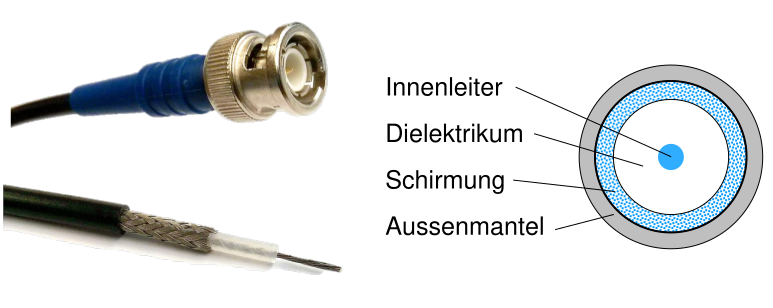
\includegraphics[width=8cm]{img/koax.png}
		\end{center}
		\caption{Koaxkabel}
		\label{fig:Koaxkabel}
\end{figure}
\paragraph{Twisted Pair Kabel}
sind weit verbreitet und gibt es in vielen Varianten. Grundsätzlich werden zwei isolierte Kabel umeinander gedreht, wobei das eine als Leiter und das andere als ``Ground'' fungiert, wodurch der Stromkreislauf geschlossen werden kann. Twisted Pair Kabel sind aufgrund ihrer geringerer Masse anfälliger auf Störungen als andere Übertragungsarten wie z.B. Koaxkabel. Dafür sind sie sehr flexibel und unheikel in der Anwendung. Die Kabel werden paarweise verdrillt um induktiven Störungen entgegen zu wirken, hier gilt: je enger die Kabel gewickelt sind, desto resistender ist die Signalübertragung. Zum Schutz vor kapazitiven Störungen werden die verdrillten Kabel Bündelweise mit einem Drahtgeflecht (gegen niederfrequente Störungen) und/oder  mit einer metallisch beschichteten Folie (gegen hochfrequente Störungen) abgeschirmt. Zudem können die verdrillten Kabelpaare individuell ebenfalls abgeschirmt werden, da sonst die Gefahr des Crosstalks besteht. Unter Crosstalk bezeichnet man die gegenseitige elektromagnetische Störung meherer Kabelpaar untereinander in einem Bündel.

Twisted Pair Kabel werden mit einer ISO-Beschriftung beschrieben, welche die angewendeten Schirmungen beschreibt. Ein Beispiel dafür ist \textbf{SF/UTP}. Das SF vor dem Schrägstrich sagt aus, dass das gesamte Bündel mit einem Geflechtschirm und einem Folienschirm geschützt ist. Das U nach dem Schirm sagt uns, dass die Aderpaare selbst ungeschirmt vor einander sind. Das TP bedeutet Twisted Pair. 
\begin{figure}[h!]
		\begin{center}
		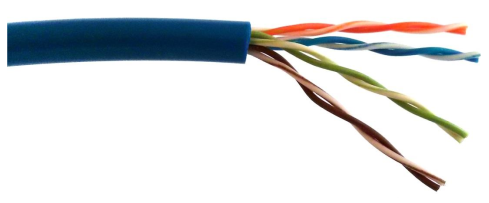
\includegraphics[width=8cm]{img/tp.png}
		\end{center}
		\caption{Twistet Pair Kabel}
		\label{fig:Twistet Pair Kabel}
\end{figure}
\subsubsection{Lichtwellenleiter}
Lichtwellenleiter verfügen über eine hohe Bandbreite und eine geringe Dämpfung. Da das Signal rein optisch übertragen wird, werden Lichtwellenleiter auch nicht durch elektromagnetische Effekte beeinflusst. Lichtwellenleiter bestehen aus einem Kernglas im Zentrum mit einem hohen Brechungsindex von 1.5, umgeben von einem Mantelglas mit einem tieferen Brechungsindex von 1.48. Umgeben ist das Glas von einer reflektierenden Ummantelung die die Dämpfung durch Absorption reduziert. Aufgrunde des Gläsernen Kerns sind Lichtwellenleiter nur bedingt flexibel und können durch zu starke Biegung brechen. Deshalb sind Lichtwellenleiter bei langen Verbindungen sehr verbreitet aber ungeeignet für die Anbindung von Endgeräten an ein Netzwerk.
\begin{figure}[h!]
		\begin{center}
		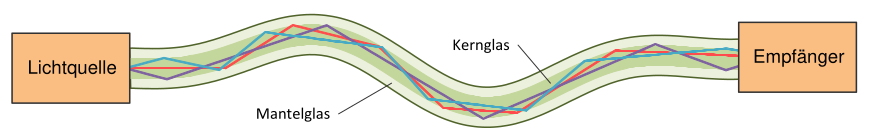
\includegraphics[width=8cm]{img/lwl2.png}
		\end{center}
		\caption{Lichtwellenleiter Querschnitt}
		\label{fig:Lichtwellenleiter Querschnitt}
\end{figure}
\paragraph{Dispersion}
bewirkt, dass sich die Übertragungsdistanz und die maximale Bandbreite gegenseitig begrenzen. Je länger die Übertragungsdistanz, desto stärker nimmt die Amplitude des Signals ab und desto länger wird ein einzelnder Impuls, wodurch sich hochfrequente Impulse bei zu langer Übertragung zu Überlagern beginnen.
\begin{figure}[h!]
		\begin{center}
		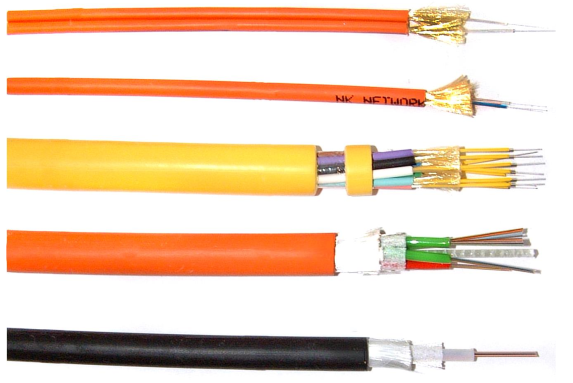
\includegraphics[width=8cm]{img/lwl.png}
		\end{center}
		\caption{Lichtwellenleiter}
		\label{fig:Lichtwellenleiter}
\end{figure}
\subsection{Layer 1 - Physical Layer}
\subsection{Layer 2 - Data Link Layer}
\subsection{Layer 3 - Network Layer}
\subsection{Layer 4 - Transport Layer}
\subsection{Layer 5 - Session Layer}
\subsection{Layer 6 - Presentation Layer}
\subsection{Layer 7 - Application Layer}

\end{document}
